\documentclass[a4paper,11pt]{article}

\usepackage[english]{babel}
\usepackage[utf8x]{inputenc}
\usepackage{amsmath}
\usepackage{graphicx}
\usepackage[margin=0.5in]{geometry}
\usepackage{caption}
\usepackage{subcaption}

\title{Convergent Cross-Mapping and Causality Detection}
\author{McCracken,Weigel}

\begin{document}
\maketitle

\abstract{
Convergent Cross-Mapping is a technique, introduced by Sugihara {\em et al.\ }\cite{Sugihara2012}, reported to be ``a necessary condition for causation'' capable of distinguishing causality from correlation in sets of time series data.  We will show that CCM correlations do not in general agree with intuitive concepts of ``driving'' and ``response'', and as such, relationships among CCM correlations should not be considered indicative of causality.  It is shown that CCM correlations can, however, be used to identify asymmetric relationships between pairs of time series data.  We introduce a 2-vector called the ``pairwise asymmetric inference'' (PAI) and present examples of its use in inferring relationships within complex systems.  The sensitivity of CCM correlations (and consequently, directed correlations) on embedding dimensions and lag times will be discussed and mitigation will be presented.
}

\section{Introduction}
Modern time series analysis includes a handful of techniques meant to discren "driving" or "cause and effect" relationships between different data sets.  These techniques have found application in a wide range of fields including neuroscience (e.g.\ \cite{Kaminski2001}), economics (e.g.\ \cite{dufour1998,dufour2006}), climatology (e.g.\ \cite{mosedale2006}), and others.  General casual relationships in time series data are also being studied in an effort to understand causality itself (e.g.\ \cite{eichler2012}).  

To date, most techniques for ``causal inference'' in time series data fall into two broad categories, those related to transfer entropy and those related to Granger causality.  Transfer entropy (introduced in \cite{Schreiber2000}) and Granger causality (introduced in \cite{granger1969}) are known to be equivalent under certain conditions \cite{Barnett2009}.  In this article, we investiagte a casual inference technique, called Convergent cross-mapping (CCM), that was recently introduced by Sugihara {\em et al.\ } in \cite{Sugihara2012}.  Currently, there is no evidence that CCM is related to either transfer entropy or Granger causality.

We will begin with a review of the work of Sugihara {\em et al.}, including working through the coupled logistic map example presented in \cite{Sugihara2012}.  We will then illustrate the dependence of CCM correlations on the embedding dimension and lag time parameters of the CCM algorithm.  Finally, we will introduce ``pairwise asymmetric inference'' (PAI) and use it to show that, even though CCM causality may not be physical caulsality, it can still be a useful tool in the analysis of complex time series data.

\section{Convergent Cross-Mapping}
CCM is described as a technique used to identify ``causality'' between time series and is intended to be useful in situations where Granger causality is known to be invalid (i.e.\ in dynamic systems that are ``nonseperable'' \cite{Sugihara2012}).  The authors state that CCM is a ``necessary condition for causation''.  It is well known \cite{Granger1980,liu2012,Roberts1985} that Granger causality is not causality as it is typically understood in physics.  It will be shown that a similar conclusion can be drawn regarding CCM causality. 

CCM is closely related to simplex projection \cite{Sugihara1990,Sugihara1990a}, which predicts a point in the times series $X$ at a time $t+1$, i.e.\ $X_{t+1}$, by using the points with the most similar histories to $X_t$.  Similarly, CCM uses points with the most similar histories to $X_t$ to estimate $Y_t$.  The CCM correlation is the squared correlation coefficient\footnote{This definition differs slightly from the original definition in \cite{Sugihara2012}, which just uses Pearson’s correlation coefficient.  We use the square of this value to avoid dealing with negative correlation values.  This subtle change in the definition does not affect the conclusions drawn in \cite{Sugihara2012}, as can be seen in our reproduction of key plots from that work.} between the original time series $Y$ and estimate of $Y$ made using the convergent cross-mapping with $X$, which is labelled as $Y|X$; i.e.\ the CCM correlation is given as 
$$
C_{YX} = \left(\rho\left(Y,Y|X\right)\right)^2\;\;,
$$
where $\rho(A,B)$ is the Pearson correlation coefficient between $A$ and $B$ \cite{}.  Any pair of times series, $X$ and $Y$, will have two CCM correlations, $C_{YX}$ and $C_{XY}$, which are compared to determine the CCM causality.  For example, Sugihara {\em et al.\ }define a difference of CCM correlations
\begin{equation}
\label{eqn:delta}
\Delta = C_{YX} - C_{XY}
\end{equation}
and use the sign of $\Delta$ to determine the CCM causality between $X$ and $Y$ \cite{Sugihara2012}.  The CCM algorithm is explained in more detail in Appendix \ref{sec:appA}.

If $X$ can be estimated from the shadow manifold of $Y$ better than $Y$ can be estimated from the shadow manifold of $X$ (e.g.\ if $\Delta < 0$), then $X$ is said to ``CCM cause'' $Y$.

\subsection{Simplified Two Population Dynamics}
\label{sec:2Pop}
Consider the example system used by Sugihara {\em et al.\ }in \cite{Sugihara2012}:
\begin{eqnarray}
\label{eqn:2pop}
X_t &=& X_{t-1}\left(r_x-r_x X_{t-1}-\beta_{xy} Y_{t-1}\right)\\
Y_t &=& Y_{t-1}\left(r_y-r_y Y_{t-1}-\beta_{yx} X_{t-1}\right)
\end{eqnarray}
where $r_x,r_y,\beta_{xy},\beta_{yx}\in\mathbf{R}\ge 0$.  This pair of equations is a specific form of the two-dimensional coupled logistic map system, which is known to be chaotic \cite{Lloyd1995}.

In this example, the CCM causality of this system is determined by sampling both the initial conditions and the dynamics parameters, calculating $\Delta$, and demonstrating the necessary convergence.  The dynamic parameters $r_x$ and $r_y$ are sampled from a normal distributions $N\left(\mu_{rx},\sigma_{rx}\right)$ and $N\left(\mu_{ry},\sigma_{ry}\right)$, respectively.  The initial conditions $X_0$ and $Y_0$ are also sampled for normal distributions, specifically $N\left(\mu_{x0},\sigma_{x0}\right)$ and $N\left(\mu_{y0},\sigma_{y0}\right)$.  The coupling parameters $\beta_{xy}$ and $\beta_{yx}$ are then varied over the interval $[10^{-6},1]$ (in steps of {\bf ????}) to produce the plots seen in Figure \ref{fig:}.

Sugihara {\em et al. }consider convergence to be critically important to determining CCM causality, identifying it as ``a key property that distinguishes causation from simple correlation'' \cite{Sugihara2012}.  Figure \ref{fig:} shows plots created with several different library lengths to illustrate the convergence of $\Delta$ for this example.  Typically, for convenience, the (approximately) converged CCM correlation values will be reported and proof of convergence will be implied, rather than shown.
\begin{figure}[ht]
\label{fig:}
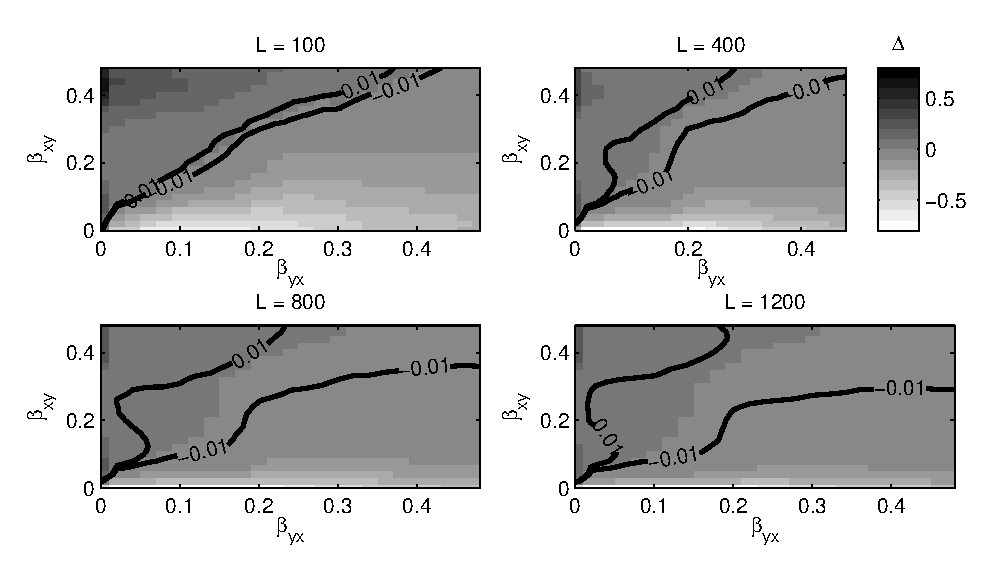
\includegraphics[scale=0.6]{Figure1.eps}
\caption{These plots show the dependence of Eqn.\ \ref{eqn:delta} on $\beta_{xy}$ and $\beta_{yx}$.  See the text for details on how these plots were created along with a discussion of the interpretation of these plots in terms of the CCM causality.}
\end{figure}
\begin{figure}[ht]
\label{fig:}
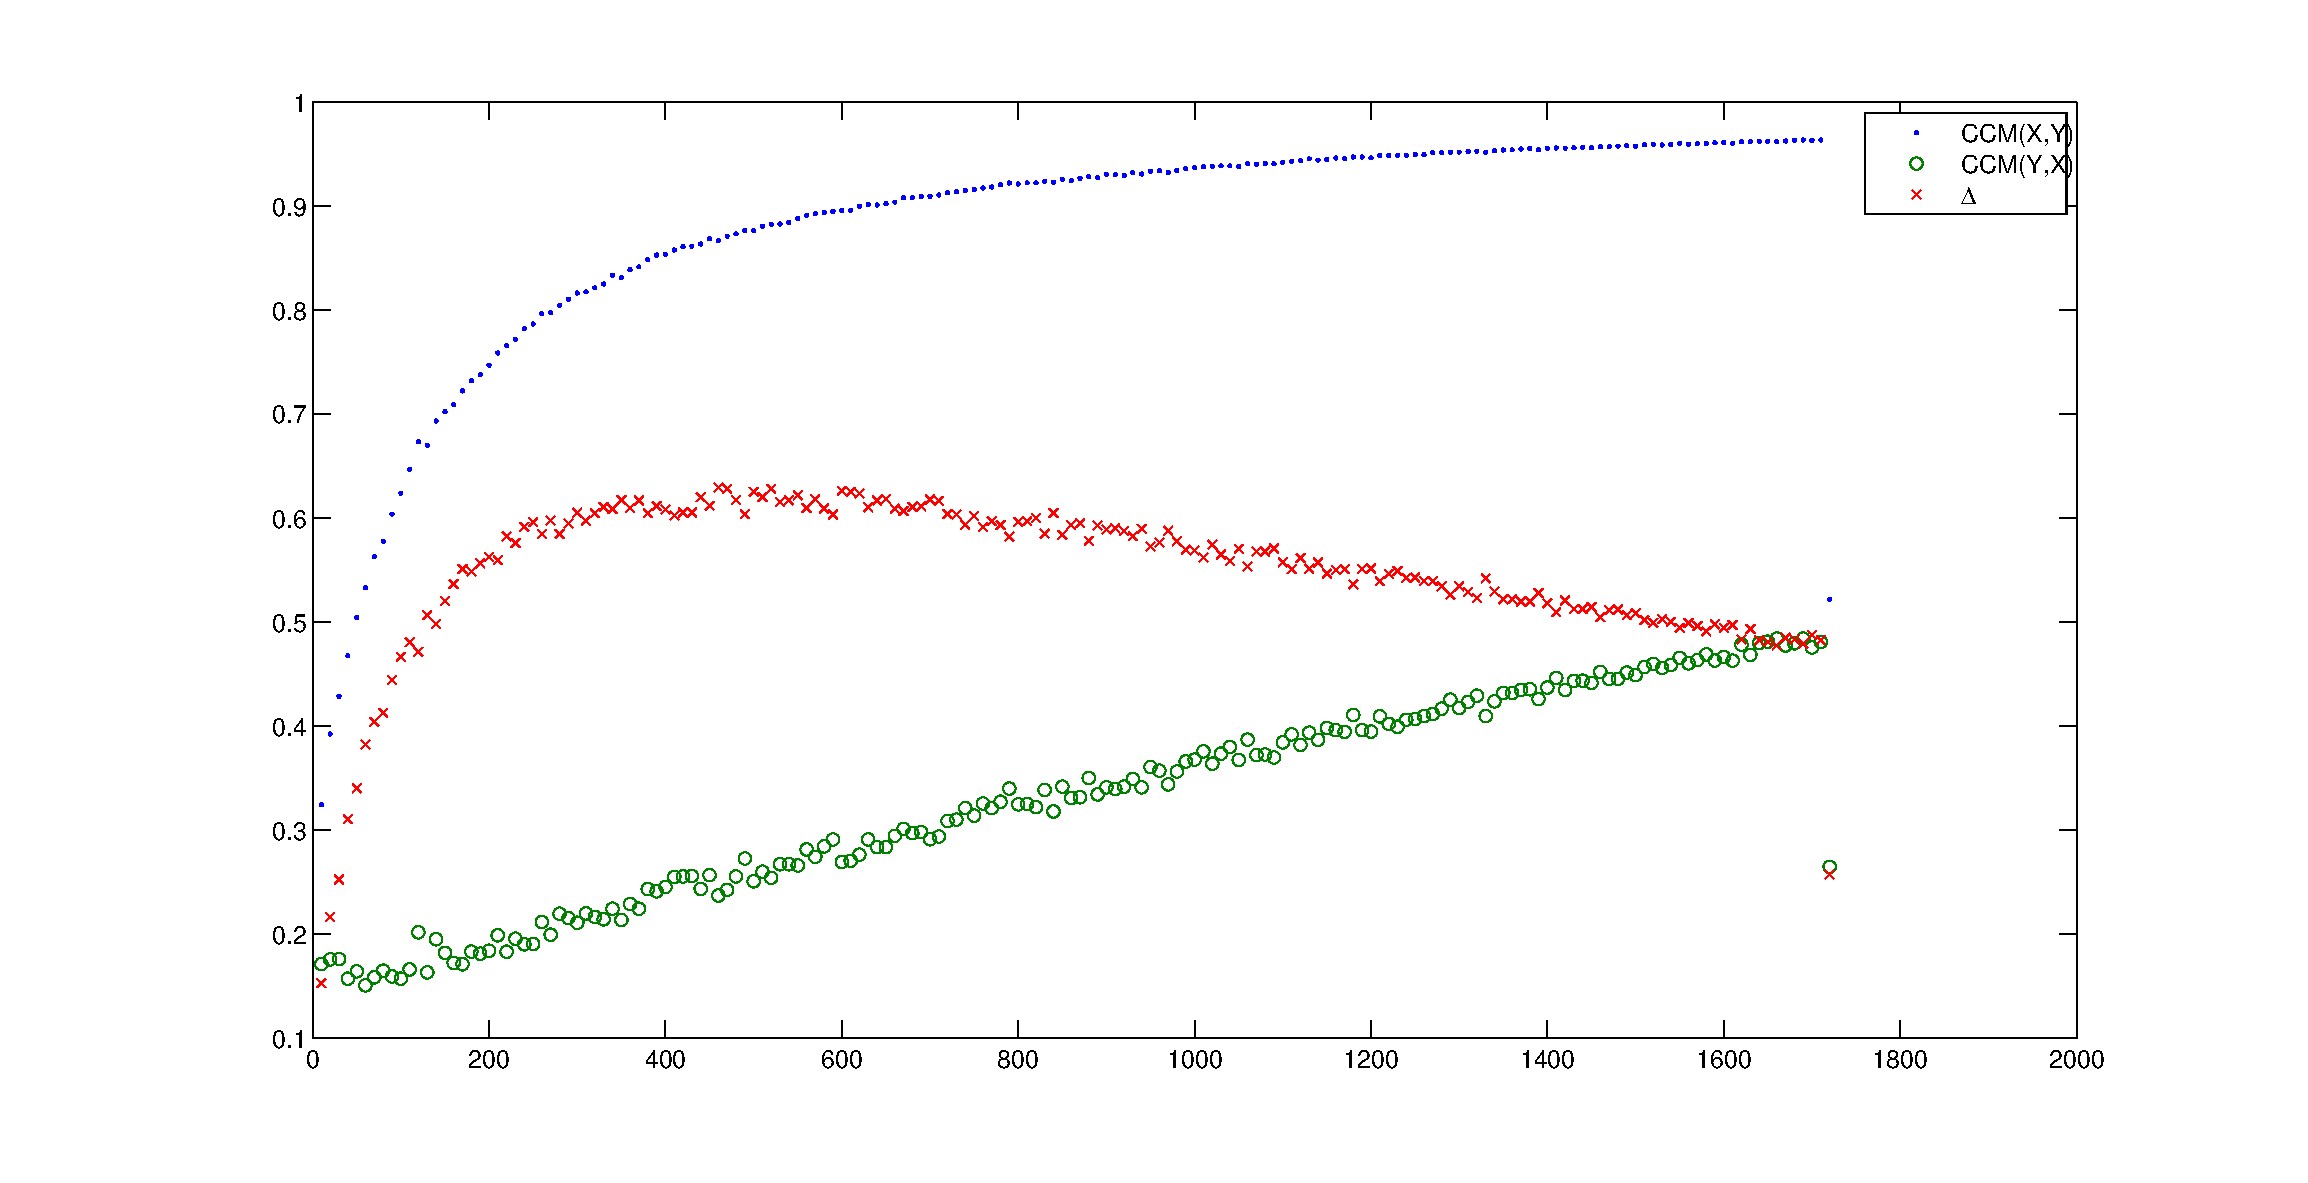
\includegraphics[scale=0.45]{RefFigure.eps}
\caption{Reference figure.}
\end{figure}

The idea is that $\beta_{xy}>\beta_{yx}$ intuitively implies $Y$ ``drives'' $X$ more than $X$ ``drives'' $Y$.  Stated more formally, $\beta_{xy}>\beta_{yx}\Rightarrow\Delta>0$, which is reported as ``$Y$ CCM causes $X$''.  Likewise, $\beta_{xy}<\beta_{yx}$ implies $X$ CCM causes $Y$ and $\beta_{xy}=\beta_{yx}$ implies no CCM causality in the system.  It will be shown below that CCM causality is not necessarily related to causality as it is typically understood in physics.

\section{Embedding Dimension and Lag Time}
The CCM algorithm depends on the embedding dimension $E$ and the lag time step $\tau$ (see Appendix \ref{sec:appA}).  Consider the simplified two population system (Eqn.\ \ref{eqn:2pop}) with $r_x=3.8$, $r_y=3.5$, $\beta_{xy}=0.01$, $\beta_{yx}=0.2$, $X_0=0.4$, and $Y_0=0.2$ with $X$ and $Y$ library lengths of $L=1000$.  Figure \ref{fig:} shows the effect of varying $E$ and $\tau$ on $\Delta$ for this system.  $E$ is varied over the interval $[2,20]$ (in steps of 1), and $\tau$ is varied over the interval $[1,50]$ (also in steps of 1).  This figure makes it clear that a statement of CCM causality (and, subsequently, that statement's agreement with ``intuition'') depends strongly upon how the CCM technique is used.
\begin{figure}[ht]
\label{fig:}
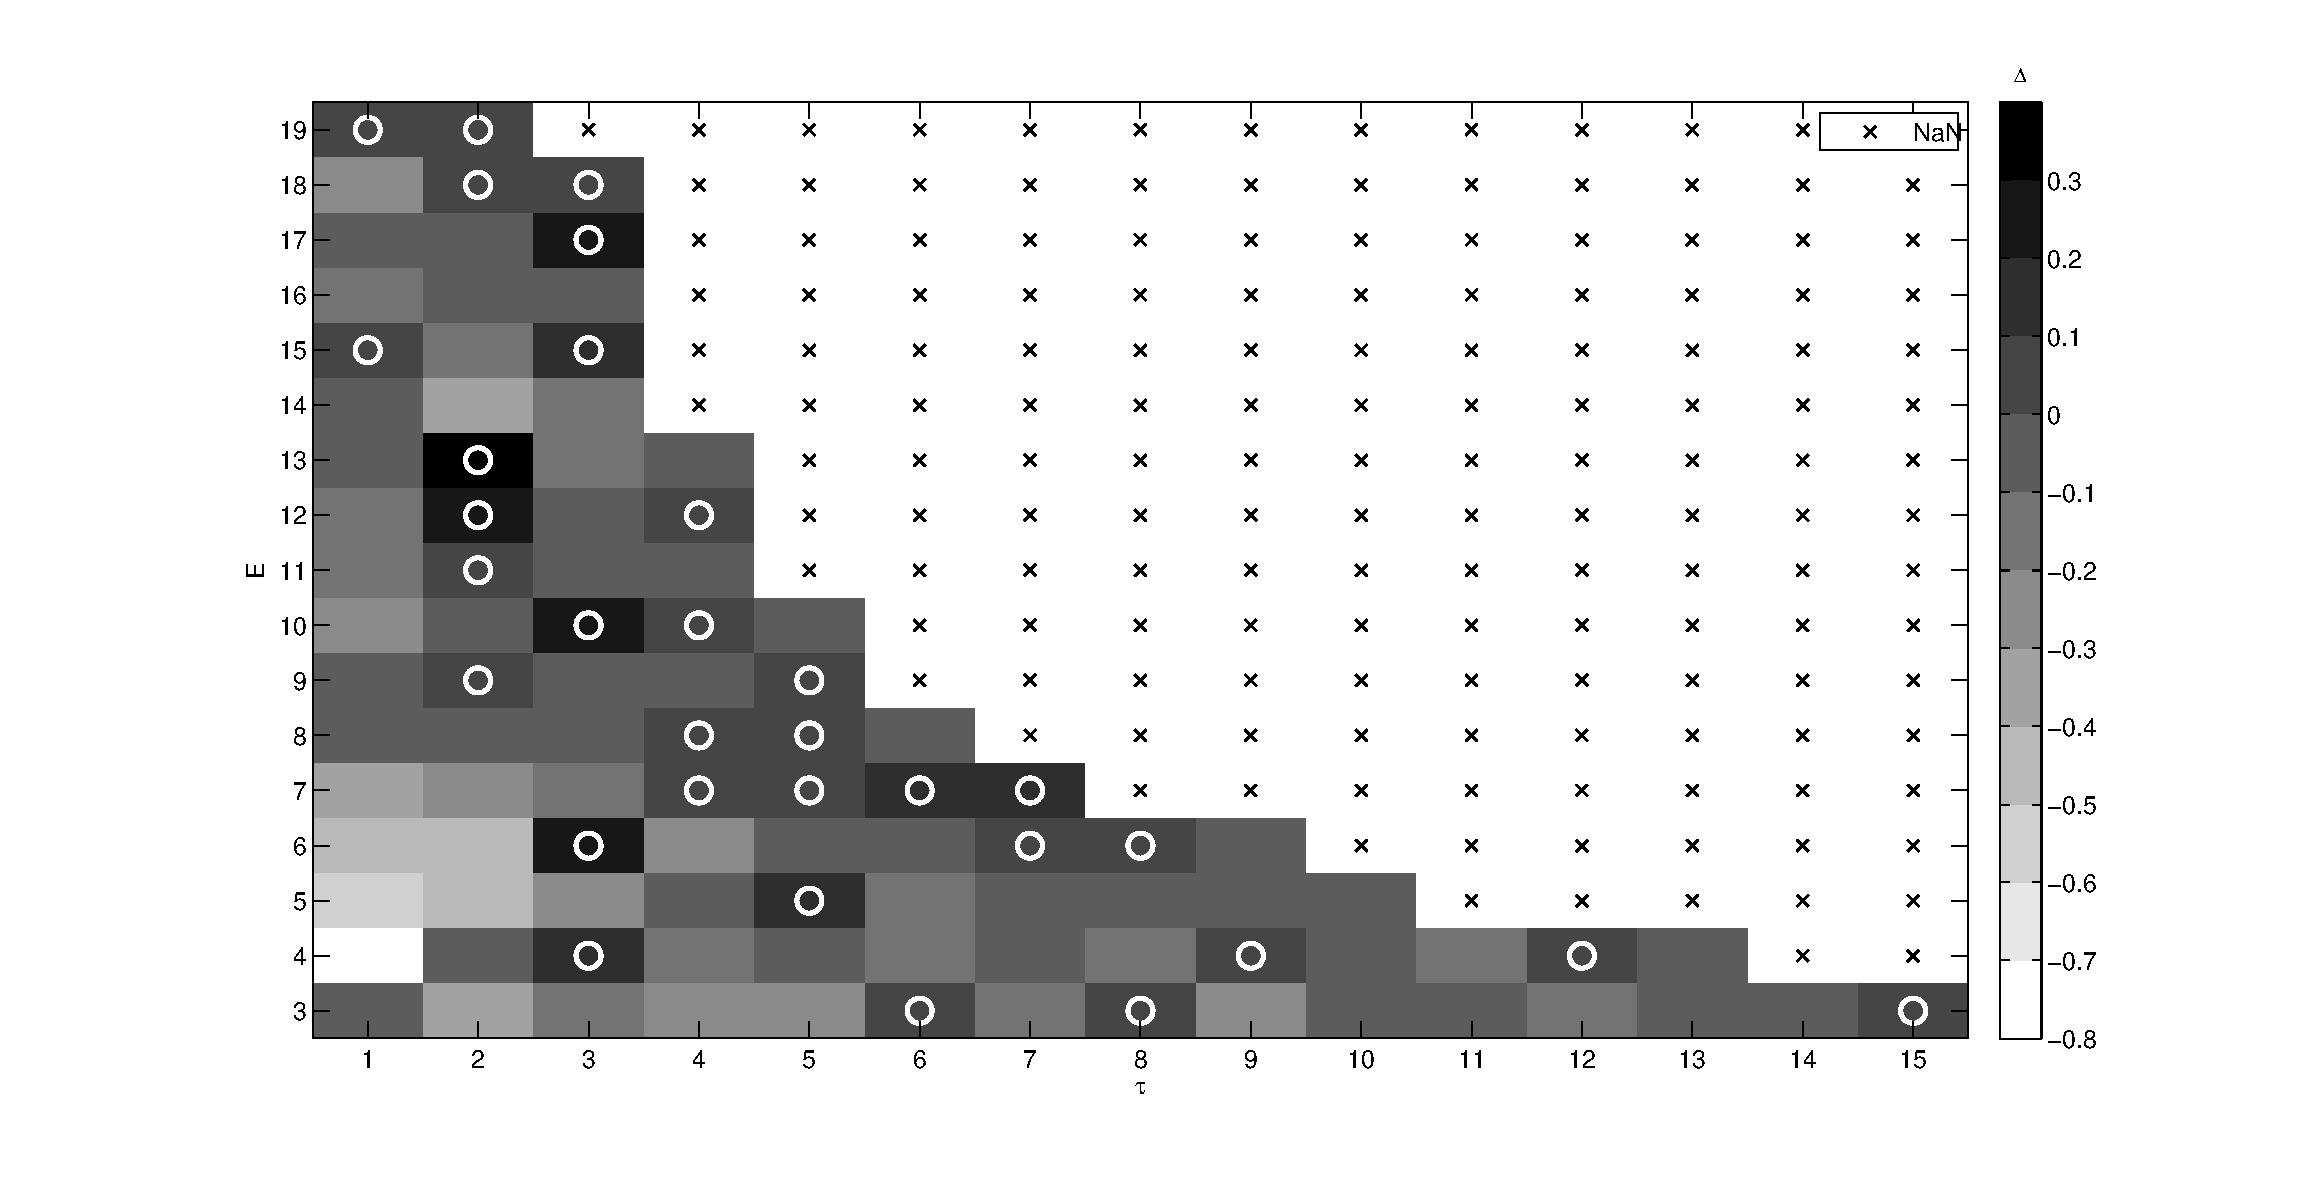
\includegraphics[scale=0.5]{Figure2.eps}
\caption{The determination of CCM causality in a system is dependent on the CCM parameters of embedding dimension $E$ and lag time step $\tau$.  This plot show the dependence of Eqn.\ \ref{eqn:delta} on $E$ and $\tau$ for the example system discussed in the text.}
\end{figure}

A dependence $E$ and $\tau$ is a feature of most state space reconstruction (SSR) methods \cite{Hong2006,vlachos2009,Small2004}.  CCM is related to state space reconstruction \cite{Sugihara2012}, so the $E$ and $\tau$ dependence seen here is not unexpected.  Sugihara {\em et al.\ }do not discuss in depth how to determine $E$ and $\tau$, but they do mention that ``optimal embedding dimensions'' are found using univariate SSR \cite{Sugihara2012} (supplementary material).  

Define the $l$-lagged autocorrelation $A_l^X$ of $X_t$ as $A_l^X=\rho\left(X_t,X_{t-l}\right)$ given $t\in[l,L]$ and $l\in[0,L/2]$ where $L$ is the library length.  The lag time step $\tau$ will be set equal to the value of $l$ that yields the maximum $l$-lagged autocorrelation; i.e.\
\begin{equation}
\tau = l \;|\; \left|A_l^X\right| = \max_l \left|A_l^X\right|\;\;.
\end{equation}
In all of the examples discussed so far, this method leads to setting $\tau=1$.  Setting $\tau$ independently of $E$ may lead to non-optimal choices for both due to their interdependence \cite{Small2004}.  This method, however, is convenient, and optimality is not required for the present study.

The embedding dimension $E$ will be determined using a method very similar to the ``false nearest neighbor'' method commonly used in SSR \cite{Kennel1992}.  The details of our method are outlined in Appendix \ref{sec:appB}.  The method requires setting a tolerance level $\delta$ and set of time steps to be checked $T$.  All of the embedding dimensions used in this work were found using $\delta=10^{-6}$ and $T=L/2$ where $L$ is the library length of the time series being investigated.

\section{PAI}
The use of Eqn.\ \ref{eqn:delta} to study CCM causality hides information present in the individual CCM correlations that may be of some use.  For example, $\Delta = 0.01$ could result from either $C_{XY} = 0.98$ and $C_{YX} = 0.99$ or $C_{XY} = 0.05$ and $C_{YX} = 0.06$.  These two different sets of CCM correlations indicate very different relationships between the times series and their shadow manifold predicted counterparts.  

Notice that the pair $\left(C_{XY},C_{YX}\right)$ is a point in the unit square.  The ``pairwise asymmetric inference'' (PAI), $\vec{P}$, is defined as a 2-vector on the unit square from the origin to the point $\left(C_{XY},C_{YX}\right)$.  The magnitude of $\vec{D}$ is 
\begin{equation}
P_m = \sqrt{C_{XY}^2+C_{YX}^2}\;\;,
\end{equation}
and its angle with the base of the square is
\begin{equation}
P_\theta = \arctan\left(\frac{C_{YX}}{C_{XY}}\right)\;\;.
\end{equation}

As an example, the directed correlation for the simplified two population example discuss in Section \ref{sec:2Pop} is shown in Figure \ref{fig:}.  The same sampling procedures described in that section were used and the coupling constants were set to $\beta_{xy}=0.02$ and $\beta_{yx}=0.1$.
\begin{figure}[ht]
\label{fig:}
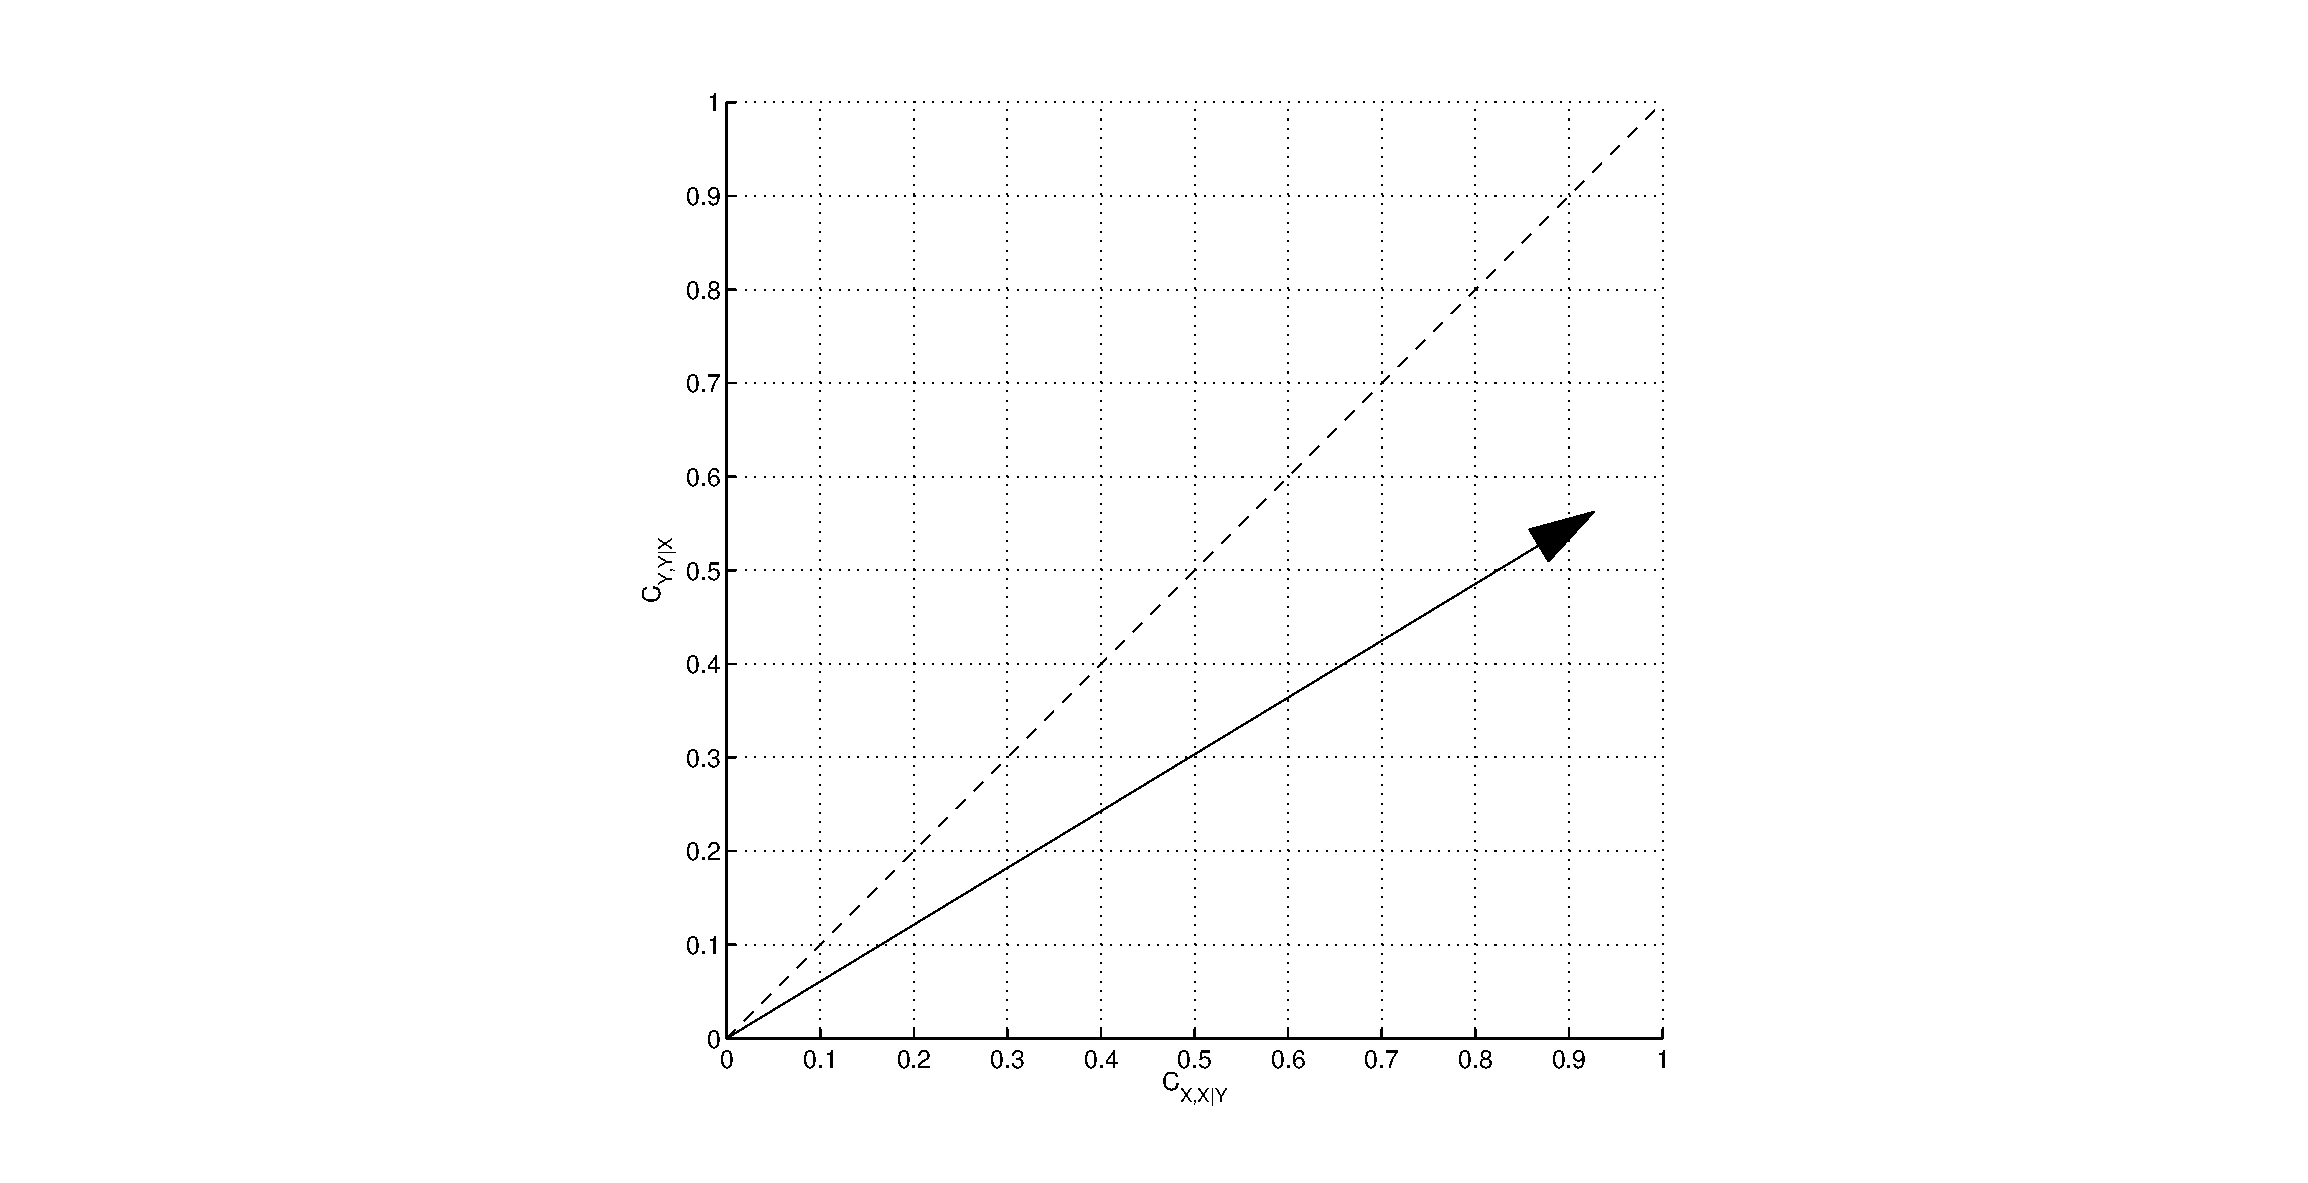
\includegraphics[scale=0.45]{Figure3.eps}
\caption{The PAI can be used to study the CCM causality in a system.  See the text for an explanation of the dynamics that yield the $\vec{D}$ shown here.}
\end{figure}
Figure \ref{fig:} shows $\vec{D}$ lies in the lower triangular quadrant on the unit square, which indicates $X$ CCM causes $Y$.  This conclusion, as discussed in Section \ref{sec:2Pop}, seems to agree with intuition.  Notice that a $\vec{D}$ aligned along the unit square bisector (i.e. the line $C_{YX}=C_{XY}$) would indicate no CCM causality in the system.

\section{Driven System Example: RL Circuit}
A circuit containing only a resistor and a inductor is described by the following differiential equation \cite{halliday2013}:
\begin{equation}
\label{eqn:it}
\frac{dI}{dt} = \frac{V(t)}{L} - \frac{R(t)}{L} I(t)\;\;,
\end{equation}
where $I(t)$ is the current at time $t$, $V(t)$ is the voltage at time $t$, $R(t)$ is the resistance at time $t$, and $L$ is the inductance.  The voltage and resistance are considered to be under the control of the experimenter.  Consider, for example, that the resistance $R$ is provided by a potentiometer controlled by the experimenter.  The inductance is considered fixed.  This scenario outline implies that the times series for $V$ and $R$ should be considered the driving time series and $I$ is the response times series.  

Consider the scenario where the voltage is described by a simple sine wave, i.e.\
\begin{equation}
\label{eqn:vt}
V(t) = \sin(t)
\end{equation}
and the resistance is given by
\begin{equation}
\label{eqn:rt}
R(t) = A\sin(\omega t + \phi) + R_0\;\;.
\end{equation}
Consider $A=R_0=0.5$ with $\omega=1$ and $\phi=0$.  These values lead to the directed correlations $\vec{D}$ in Figure \ref{fig:}.  
\begin{figure}[ht]
\label{fig:}
\caption{The PAI of an RL circuit with $V(t)$ and $R(t)$ given by Eqn. \ref{eqn:vt} and Eqn. \ref{eqn:rt}, respectively, can be calculated for each of the three parameters pairs; i.e.\ $(V,I)$, $(R,I)$, and $(V,R)$.  The parameters used to produce these plots are explained in the text.  Notice that these results imply {\bf ????}, which agrees with the physical "intuition" for this situation.}
\end{figure}
These PAIs seem to imply CCM causality is at least representative of physical causality.  Notice, however, that changing the phase, $\omega$, of the resistance $R(t)$ can lead to situations that do not support the intuitive result of $R$ CCM causes $I$.  For example, consider $A=R_0=\omega=0.5$.  These values lead the the PAIs in Figure \ref{fig:}.
\begin{figure}[ht]
\label{fig:}
\caption{The PAIs of Figure \ref{fig:} change dramatically when the phase between $R(t)$ and $V(t)$ is changed.  See the text for the parameters used to produce $\vec{D}$.}
\end{figure}

Consider the situation where the voltage is driven with the sinusoidal signal shown in Eqn. \ref{eqn:vt} and the resistance is driven by the triangular pulse 
\begin{equation}
\label{eqn:rttrig}
???
\end{equation}
where $\ldots$.  Such a scenario leads to the PAIs shown in Figure \ref{fig:}.
\begin{figure}[ht]
\label{fig:}
\caption{The PAIs of the RL circuit system with $V(t)$ given by Eqn. \ref{eqn:vt} and $R(t)$ given by Eqn.\ \ref{eqn:rttrig}.}
\end{figure}
These results imply $V$ CCM causes $I$ as expected, but they also imply $I$ CCM causes $R$ and $V$ CCM causes $R$ which obeys transitivity but seems counter-intuitive.  These results seem to imply that the voltage is the primary driver of the system and can, under certain scenarios, even be seen as a ``driver'' of the resistance through the current.  Consider approximating Eqn. \ref{eqn:it} as
\begin{equation}
\dot{I} = \frac{V}{L} - \frac{R}{L} I\Rightarrow I_{t+1}-I_t = \frac{V_t}{L} - \frac{R_t}{L} I_t\;\;.
\end{equation}
Rearranging leads to
\begin{eqnarray}
I_{t+1} &=& \frac{V_t}{L}+I_t\left(1-\frac{R_t}{L}\right)\;\;,\\
V_t &=& L\left(I_{t+1}-I_t\left(1-\frac{R_t}{L}\right)\right)\;\;,
\end{eqnarray}
and
\begin{equation}
R_t = L\left(I_t-I_{t+1}+\frac{V_t}{L}\right)\;\;.
\end{equation}
These equations imply that if the amplitude of the voltage is significantly larger than both the resistance and the current, then it can appear to drive both the current and the resistance, as seen above.

These examples help put a fine point on the problem of using language should as ``driving'' and ``causality'' to describe the relationship indicated by the PAI (and CCM causality in general).  If the voltage, resistance, and current were all completely out of the experimenter's control and the only data available is the time series described above.  Then, it is reasonable that certain scenarios would allow the voltage to be used to predict both the resistance and the current because the voltage physically drives the current and shares a similar, repetitive mathematical structure with the resistance.  The prediction ability of the voltage for the two quantities may come from different mechanisms (i.e.\ physical driving or mathematical structure), but the prediction ability itself is what is of interest to us here.  It is not reasonable to state that the voltage physically drives the resistance in this particular case because by construction, the voltage and the resistance are independent.  

\section{PAI and Non-Linear Data Sets}
The PAI does not need a physical causality interpretation to be useful.  It is can helpful in inferring relationships between time series from complicated, non-linear dynamics.  

For example, consider the extension of the simplified two population example presented in Section \ref{sec:2Pop} to a ``three population'' system as follows:
\begin{eqnarray}
X_{t+1} &=& X_t\left(r_x-r_x X_t-B_{xy} Y_t-B_{xz} Z_t\right)\\
Y_{t+1} &=& Y_t\left(r_y-r_y Y_t-B_{yx} X_t-B_{yz} Z_t\right)\\
Z_{t+1} &=& Z_t\left(r_z-r_z Z_t-B_{zx} X_t-B_{zy} Y_t\right)
\end{eqnarray}
where $r_x,r_y,r_z,\beta_{xy},\beta_{yx},\beta_{xz},\beta_{zx},\beta_{zy},\beta_{yz}\in\mathbf{R}\ge 0$.  There is no readily apparent physical intuition for this system unlike the two population example (which was, likewise, non-linear).  For instance, if $\beta_{xz}=\beta_{}$ {\bf write this to specifically reflect the example you plan on plotting.}

\section{Conclusion}
{\bf Remember to state $E$ and $\tau$ for all the plots!}

A reasonable interpretation of the PAI and CCM causality is as the identification (and quantification) of asymmetrical prediction capability between pairs of time series data.

A set of three time series data sets $X$, $Y$, and $Z$, would have three directed correlations (which is pairwise in the data sets by definition).  Each of the three directed correlations would determine the CCM causality as, for example, whether $X$ CCM causes $Y$, $Y$ CCM causes $X$, or ``there is no CCM causality in this system''.  The relationship stated using the phrase ``CCM causes'' indicates which time series history in the pair of data sets is the better predictor of its partner.  For example, the statement ``$X$ CCM causes $Y$'' indicates the histories (i.e.\ delay vectors) of $Y_t$ are better predictors of $X_t$ than the histories of $X_t$ are of $Y_t$.  Such information can be useful, but should not be confused with physical causality.
\section{Appendix A: CCM Algorithm}
\label{sec:appA}
A description of this algorithm is also available in \cite{Sugihara2012} (supplementary materials).  It is elucidating to partition the CCM algorithm into five distinct (though related) steps:
\begin{enumerate}
\item Create the shadow manifold for $X$, called $\tilde{X}$
\item Find the nearest neighbours to $\tilde{X}_t$
\item Use the nearest neighbours to create weights
\item Use the weights to estimate $Y$, called $Y|X$
\item Find the correlation between $Y$ and $Y|X$ 
\end{enumerate}
The steps vary in complexity and are explained in more detail below.

\subsection{Create $\tilde{X}$}
Given an embedding dimension $E$, the shadow manifold of $X$, called $\tilde{X}$, is created by associating an $E$-dimensional vector to each point $X_t$ that is constructed as $\vec{X}_t=(X_t,X_{t-\tau},X_{t-2\tau},\ldots,X_{t-(E-1)\tau}$ (this vector is often called a ``delay vector'').  The first such vector is created at $t=1+(E-1)\tau\equiv t_s$ and the last is at $t=L\equiv t_l$ where $L$ is the time series length (or ``library length'').  

\subsection{Find Nearest Neighbours}
The minimum number of points required for a bounding simplex in an $E$-dimensional space is $E+1$ (find a non-Sugihara reference for this statement).  Thus, the nearest neighbour search results is a set of distances $\{d_1,d_2,\ldots,d_{E+1}\}$ and an associated set of times $\{t_1,t_2,\ldots,t_{E+1}\}$ (where the subscript 1 denotes the closest neighbour, 2 denotes the next closest neighbour, and so on).  The distances from $\vec{X}_t$ are defined as
$$
d_i = D\left(\vec{X}_t,\vec{X}_{t_i}\right)\;\;,
$$
where $D(\vec{a},\vec{b})$ is the Euclidean distance between vectors $\vec{a}$ and $\vec{b}$.

\subsection{Create Weights}
Each nearest neighbour will be used to find an associated weight.  The unnormalized weights are defined as
$$
u_i = e^{-\frac{d_i}{d_1}}\;\;.
$$
The weights are defined as
$$
w_i = \frac{u_i}{N}\;\;,
$$
where the normalization factor is given as
$$
N = \sum_j u_j\;\;.
$$

\subsection{Find $Y|X$}
A point $Y_t$ in $Y$ can be estimated using the (normalized) distances to the points in $X$ using the weights calculated above.  This estimate is calculated as
$$
Y_t|X = \sum_i w_i Y_{t_i}\;\;.
$$

\subsection{Find the Correlation}
The CCM correlation is defined as 
$$
C_{YX} = \left(\rho\left(Y,Y|X\right)\right)^2\;\;,
$$
where $\rho_{A,B}$ is the standard Pearson's correlation coefficient between $A$ and $B$.  It can be seen from the above algorithm that $X=Y \Rightarrow C_{YX}=C_{XY}$, but in general, $C_{YX}\neq C_{XY}$.  

\section{Appendix B: Determining $E$}
\label{sec:appB}
The algorithm we use for determining the embedding dimension $E$ can be outlined as follows:
\begin{enumerate}
\item Embed $X$ in a shadow manifold $\tilde{X}$ with dimension $E$ (see Appendix \ref{sec:appA})
\item Record the weights $\{w^E_i\}$ of the $E+1$ nearest neighbors to $\tilde{X}_t$ 
\item Repeat steps 1 and 2 for $E=E+1$
\item Stop when $\exists w^E_i < \delta$
\item Record $E$ (i.e.\ the embedding dimension for which the above iteration is halted) as $E^H_t$
\item Repeat steps 1-4 for all $t\le T$ where $T$ is dependent on the library length $L$ of $X$ 
\item Find the mode of $\{E_t^H\}$
\end{enumerate}
This algorithm requires the selection of some $\delta$ and $T$.  Both parameters are usually chosen to be ``sufficiently small'' while still being computationally tractable.  

Notice that all subjectivity can be removed from this algorithm by recording the locations $\tilde{t}^E_i$ associated to each $w^E_i$ and setting the halt criterion in Step 4 to ``Stop when $\{\tilde{t}^E_i\}\not \subset \{\tilde{t}^{E+1}_i\}$''; i.e.\ stop when, for example, a nearest neighbour of $\tilde{X}_t$ given $E=3$ is no longer a nearest neighbor when $E=4$.  The set of time steps $T$ can be set to $\tilde{L}$, the library length of $\tilde{X}$.  These modifications will remove the need to set any (possibly arbitrary) parameters such as $\delta$ and $T$, but the algorithm will become much more computationally expensive.

It is assumed that the lag time step $\tau$ is determined (e.g.\ with the autocorrelation method discussed in the main text) before this algorithm begins.  This algorithm can be modified to concurrently determine $\tau$ and $E$ by repeating Steps $1-3$ for successive iterations of $\tau$ and recording the halting values of both $E$ and $\tau$ in Step 5.  But, again, such a modification will significantly increase the computational cost of the algorithm.

\bibliographystyle{plain}
\bibliography{main}

\end{document}

